\begin{slide}
    \begin{block}{Virtual Machine}
        Execute the bytecode instructions generated.
    \end{block}
    \vfill
    \slidecaps{IMPLEMENTED}
    \begin{itemize}
        \item A call stack.
        \item A value stack to pass parameters.
        \item Automatic call to the \texttt{main} function with \texttt{argv} argument.
    \end{itemize}
\end{slide}
\begin{slide}
    \begin{figure}[H]
        \centering
        \begin{subtable}{0.5\textwidth}
            \begin{minted}{cpp}
fun mul(a: int): int {
    return a * 2
}

fun main(argv: [string]) {
    print mul(10)
}
            \end{minted}
        \caption{Input program}
        \end{subtable}
        \begin{subtable}{0.45\textwidth}
            \only<1>{
                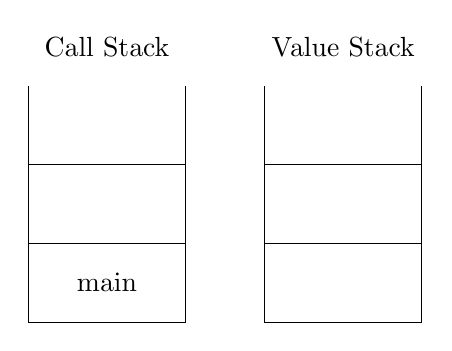
\begin{tikzpicture}
                    % Labels
                    \node at (1, 3.5) {Call Stack};
                    \node at (4, 3.5) {Value Stack};
                    % Stack
                    \draw[] (0, 0) -- (2, 0);
                    \draw[] (0, 1) -- (2, 1);
                    \draw[] (0, 2) -- (2, 2);
                    \draw[] (0, 0) -- (0, 3);
                    \draw[] (2, 0) -- (2, 3);
                    % Elements
                    \node at (1, 0.5) {main};
                    % Stack
                    \draw[] (3, 0) -- (5, 0);
                    \draw[] (3, 1) -- (5, 1);
                    \draw[] (3, 2) -- (5, 2);
                    \draw[] (3, 0) -- (3, 3);
                    \draw[] (5, 0) -- (5, 3);
                    % Elements
                \end{tikzpicture}
            }
            \only<2>{
                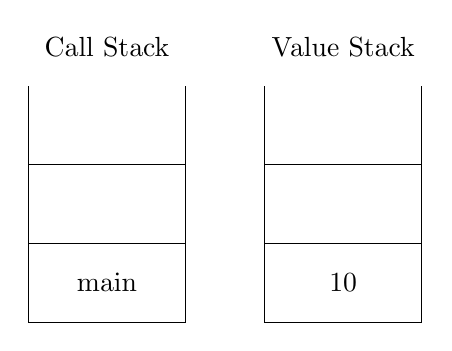
\begin{tikzpicture}
                    % Labels
                    \node at (1, 3.5) {Call Stack};
                    \node at (4, 3.5) {Value Stack};
                    % Stack
                    \draw[] (0, 0) -- (2, 0);
                    \draw[] (0, 1) -- (2, 1);
                    \draw[] (0, 2) -- (2, 2);
                    \draw[] (0, 0) -- (0, 3);
                    \draw[] (2, 0) -- (2, 3);
                    % Elements
                    \node at (1, 0.5) {main};
                    % \node at (1, 1.5) {mul};
                    % Stack
                    \draw[] (3, 0) -- (5, 0);
                    \draw[] (3, 1) -- (5, 1);
                    \draw[] (3, 2) -- (5, 2);
                    \draw[] (3, 0) -- (3, 3);
                    \draw[] (5, 0) -- (5, 3);
                    % Elements
                    \node at (4, 0.5) {10};
                \end{tikzpicture}
            }
            \only<3>{
                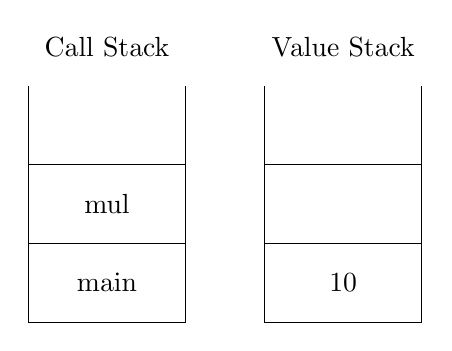
\begin{tikzpicture}
                    % Labels
                    \node at (1, 3.5) {Call Stack};
                    \node at (4, 3.5) {Value Stack};
                    % Stack
                    \draw[] (0, 0) -- (2, 0);
                    \draw[] (0, 1) -- (2, 1);
                    \draw[] (0, 2) -- (2, 2);
                    \draw[] (0, 0) -- (0, 3);
                    \draw[] (2, 0) -- (2, 3);
                    % Elements
                    \node at (1, 0.5) {main};
                    \node at (1, 1.5) {mul};
                    % Stack
                    \draw[] (3, 0) -- (5, 0);
                    \draw[] (3, 1) -- (5, 1);
                    \draw[] (3, 2) -- (5, 2);
                    \draw[] (3, 0) -- (3, 3);
                    \draw[] (5, 0) -- (5, 3);
                    % Elements
                    \node at (4, 0.5) {10};
                \end{tikzpicture}
            }
            \only<4>{
                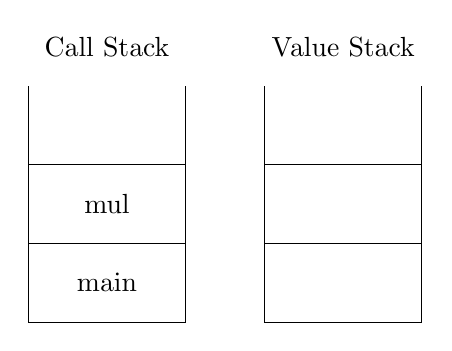
\begin{tikzpicture}
                    % Labels
                    \node at (1, 3.5) {Call Stack};
                    \node at (4, 3.5) {Value Stack};
                    % Stack
                    \draw[] (0, 0) -- (2, 0);
                    \draw[] (0, 1) -- (2, 1);
                    \draw[] (0, 2) -- (2, 2);
                    \draw[] (0, 0) -- (0, 3);
                    \draw[] (2, 0) -- (2, 3);
                    % Elements
                    \node at (1, 0.5) {main};
                    \node at (1, 1.5) {mul};
                    % Stack
                    \draw[] (3, 0) -- (5, 0);
                    \draw[] (3, 1) -- (5, 1);
                    \draw[] (3, 2) -- (5, 2);
                    \draw[] (3, 0) -- (3, 3);
                    \draw[] (5, 0) -- (5, 3);
                    % Elements
                    % \node at (4, 0.5) {10};
                \end{tikzpicture}
            }
            \only<5>{
                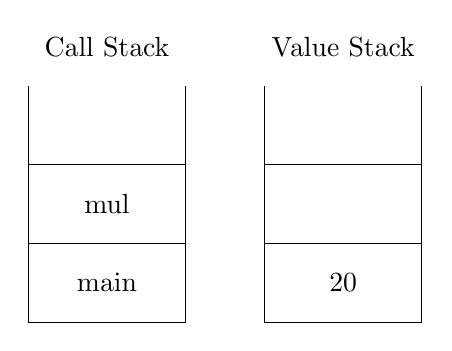
\begin{tikzpicture}
                    % Labels
                    \node at (1, 3.5) {Call Stack};
                    \node at (4, 3.5) {Value Stack};
                    % Stack
                    \draw[] (0, 0) -- (2, 0);
                    \draw[] (0, 1) -- (2, 1);
                    \draw[] (0, 2) -- (2, 2);
                    \draw[] (0, 0) -- (0, 3);
                    \draw[] (2, 0) -- (2, 3);
                    % Elements
                    \node at (1, 0.5) {main};
                    \node at (1, 1.5) {mul};
                    % Stack
                    \draw[] (3, 0) -- (5, 0);
                    \draw[] (3, 1) -- (5, 1);
                    \draw[] (3, 2) -- (5, 2);
                    \draw[] (3, 0) -- (3, 3);
                    \draw[] (5, 0) -- (5, 3);
                    % Elements
                    \node at (4, 0.5) {20};
                \end{tikzpicture}
            }
            \only<6>{
                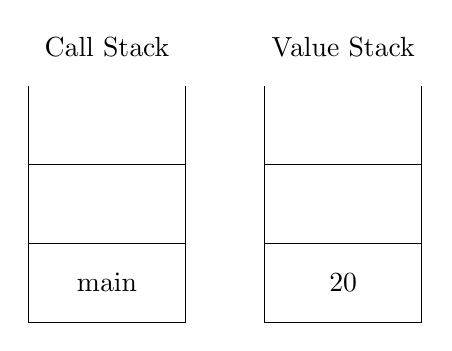
\begin{tikzpicture}
                    % Labels
                    \node at (1, 3.5) {Call Stack};
                    \node at (4, 3.5) {Value Stack};
                    % Stack
                    \draw[] (0, 0) -- (2, 0);
                    \draw[] (0, 1) -- (2, 1);
                    \draw[] (0, 2) -- (2, 2);
                    \draw[] (0, 0) -- (0, 3);
                    \draw[] (2, 0) -- (2, 3);
                    % Elements
                    \node at (1, 0.5) {main};
                    % Stack
                    \draw[] (3, 0) -- (5, 0);
                    \draw[] (3, 1) -- (5, 1);
                    \draw[] (3, 2) -- (5, 2);
                    \draw[] (3, 0) -- (3, 3);
                    \draw[] (5, 0) -- (5, 3);
                    % Elements
                    \node at (4, 0.5) {20};
                \end{tikzpicture}
            }
            \only<7>{
                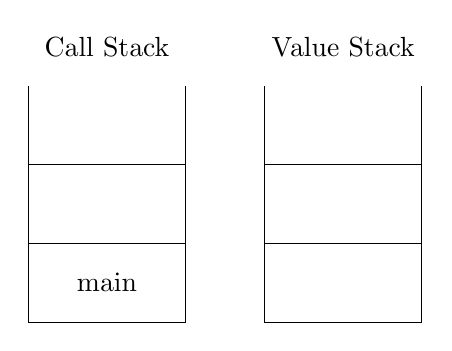
\begin{tikzpicture}
                    % Labels
                    \node at (1, 3.5) {Call Stack};
                    \node at (4, 3.5) {Value Stack};
                    % Stack
                    \draw[] (0, 0) -- (2, 0);
                    \draw[] (0, 1) -- (2, 1);
                    \draw[] (0, 2) -- (2, 2);
                    \draw[] (0, 0) -- (0, 3);
                    \draw[] (2, 0) -- (2, 3);
                    % Elements
                    \node at (1, 0.5) {main};
                    % Stack
                    \draw[] (3, 0) -- (5, 0);
                    \draw[] (3, 1) -- (5, 1);
                    \draw[] (3, 2) -- (5, 2);
                    \draw[] (3, 0) -- (3, 3);
                    \draw[] (5, 0) -- (5, 3);
                    % Elements
                \end{tikzpicture}
            }
        \caption{Stacks}
        \end{subtable}
    \caption{Stack usage on program execution}
    \end{figure}
\end{slide}
